\documentclass{beamer}

\makeatletter
\def\input@path{{Padova/}}
\makeatother

\usetheme{Padova}

\graphicspath{ {images/} }

\title{Migliorare la Business Intelligence con l'AI}
\subtitle{Discussione di Laurea Triennale in Informatica}
\author{Riccardo Stefani}
\date{23 Luglio 2025}


\begin{document}

	\maketitle

	\begin{frame}{Indice}
		\tableofcontents
	\end{frame}


	\section{Introduzione}

	\begin{frame}{Introduzione - Oribea}
		\textbf{Startup innovativa} fondata nel \textbf{2024} a \textbf{San Marino}

		\begin{columns}
			\begin{column}{0.5\textwidth}
				\begin{alertblock}{Mission}
					\begin{itemize}
						\item Soluzioni \textbf{AI avanzate}
						\item Migliorare \textbf{efficienza aziendale}
						\item Focus su \textbf{LLM}
						\item \textbf{Agenti intelligenti}
					\end{itemize}
				\end{alertblock}
			\end{column}
			\begin{column}{0.5\textwidth}
				\begin{exampleblock}{Prodotti principali}
					\begin{itemize}
						\item Automazione \textbf{processi aziendali}
						\item \textbf{AI Task Builder}
						\item \textbf{AI Chatbot Builder}
					\end{itemize}
				\end{exampleblock}
			\end{column}
		\end{columns}

		\begin{figure}[h]
			\centering
			
\includegraphics[width=0.5\textwidth]{oribea-logo.png}
		\end{figure}
	\end{frame}

	\begin{frame}{Introduzione - Il progetto}
		\textbf{Scopo}: Automatizzare la \textbf{Business Intelligence} per \textbf{e-commerce}

		\begin{columns}
			\begin{column}{0.5\textwidth}
				\begin{block}{Analisi delle vendite}
					\begin{itemize}
						\item \textbf{Input:} Dati di vendite di e-commerce (\textbf{elenco degli acquisti})
						\item \textbf{Output:} Report automatico con \textbf{statistiche} e \textbf{grafici}
					\end{itemize}
				\end{block}
			\end{column}
			\begin{column}{0.5\textwidth}
				\begin{block}{Sistema di raccomandazione}
					\begin{itemize}
						\item \textbf{Input:} \textbf{Storico acquisti} clienti-prodotti, e \textbf{nomi significativi} dei prodotti
						\item \textbf{Output:} Raccomandazioni personalizzate di \textbf{prodotti} e \textbf{clienti}
					\end{itemize}
				\end{block}
			\end{column}
		\end{columns}

		\begin{alertblock}{Motivazione personale}
			Approfondire soluzioni \textbf{AI} per \textbf{analisi dati} e \textbf{sistemi di raccomandazione}
		\end{alertblock}
	\end{frame}


	\section{Analisi delle vendite}

	\begin{frame}{Analisi delle vendite - L'idea}
		L'idea di \textbf{analisi delle vendite} prevede di fornire un sistema automatizzato che generi:

		\begin{columns}
			\begin{column}{0.6\textwidth}
				\begin{itemize}
					\item \textbf{Statistiche utili}
					\item \textbf{Grafici}
					\item \textbf{Resoconto dell'andamento} tramite LLM
				\end{itemize}
			\end{column}
			\begin{column}{0.4\textwidth}
				\begin{figure}
					\centering
					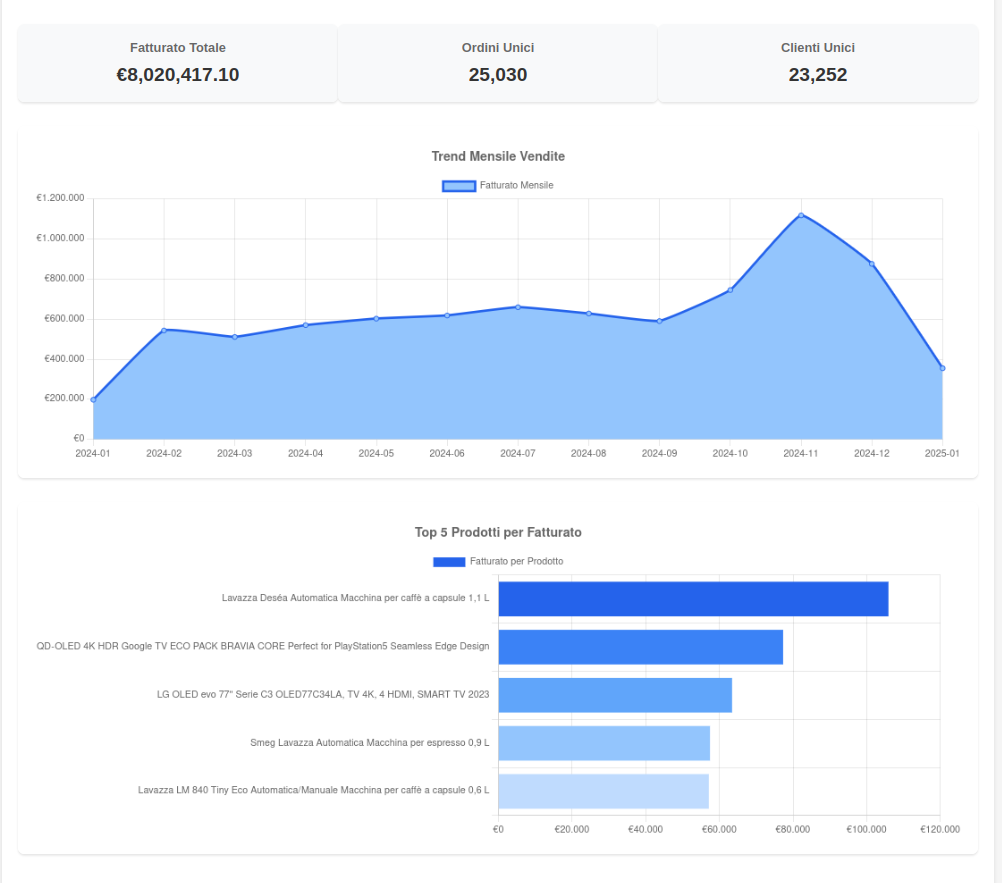
\includegraphics[width=\textwidth]{Oribea - Esempio di report delle vendite.png}
				\end{figure}
			\end{column}
		\end{columns}

		\vspace{0.5em}
		Oribea ha fornito un \textbf{prototipo} di analisi delle vendite compiuta \textbf{manualmente}, visibile in figura, come base da cui prendere \textbf{esempio} per lo sviluppo della \textbf{soluzione automatizzata}.
	\end{frame}

	\begin{frame}{Analisi delle vendite - Pipeline per la\\ generazione del report}
		\textbf{Pipeline} di elaborazione per l'\textbf{analisi automatizzata} dei dati di vendita e la \textbf{generazione del report}:

		\begin{figure}
			\centering
			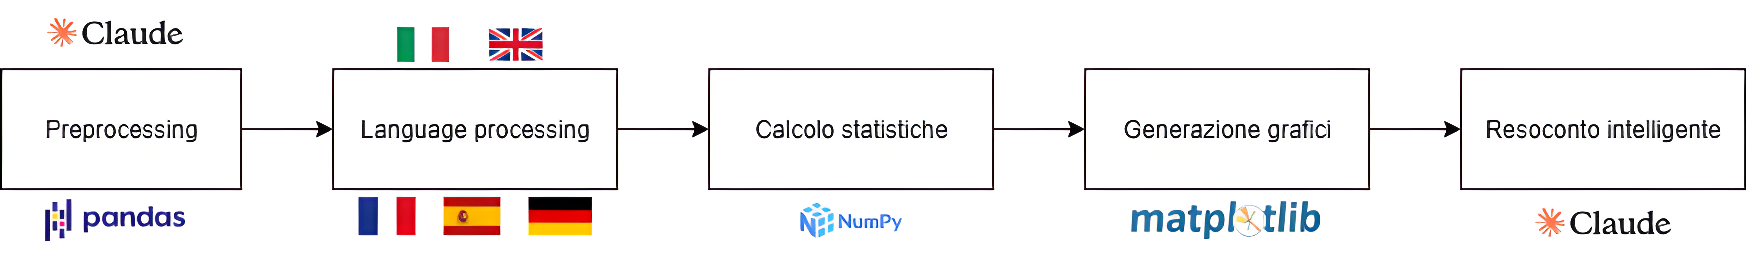
\includegraphics[width=\textwidth]{Diagramma pipeline analisi delle vendite.png}
		\end{figure}
	\end{frame}

	\begin{frame}{Analisi delle vendite - Formati di output\\ del report}
		\textbf{Output dell'analisi}: Il report generato viene presentato all'utente in \textbf{multipli formati}:

				\begin{columns}
					\begin{column}{0.33\textwidth}
						\begin{alertblock}{PDF}
							Formato \textbf{professionale} per archiviazione e condivisione
						\end{alertblock}
						\begin{figure}
							\centering
							
\includegraphics[width=0.7\textwidth]{Diagramma generazione report PDF ReportLab.png}
						\end{figure}
					\end{column}
					\begin{column}{0.33\textwidth}
						\begin{exampleblock}{HTML}
							Visualizzazione \textbf{interattiva} e responsiva nel browser
						\end{exampleblock}
						\begin{figure}
							\centering
							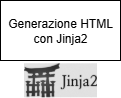
\includegraphics[width=0.7\textwidth]{Diagramma generazione report HTML Jinja2.png}
						\end{figure}
					\end{column}
					\begin{column}{0.33\textwidth}
						\begin{block}{Email}
							\textbf{Invio automatico} del report alla mail dell'utente
						\end{block}
						\begin{figure}
							\centering
							
\includegraphics[width=0.95\textwidth]{Diagramma invio report via mail SMTP.png}
						\end{figure}
					\end{column}
				\end{columns}
	\end{frame}


	\section{Sistema di raccomandazione}

	\begin{frame}{Sistema di raccomandazione - L'idea}
		\begin{columns}
			\begin{column}{0.6\textwidth}
				\begin{alertblock}{Obiettivo}
					Combinare i vantaggi del \textbf{Collaborative Filtering} con quelli della \textbf{similarità basata su contenuto} per ottenere raccomandazioni più accurate e robuste.
				\end{alertblock}

				\begin{exampleblock}{Approccio}
					Implementazione di un algoritmo di \textbf{Rank Fusion}, utilizzando in particolare il \textbf{Reciprocal Rank Fusion (RRF)}, per combinare efficacemente i risultati dei due sistemi, archiviati come \textbf{matrici}.
				\end{exampleblock}
			\end{column}
			\begin{column}{0.4\textwidth}
				\begin{figure}
					\centering
					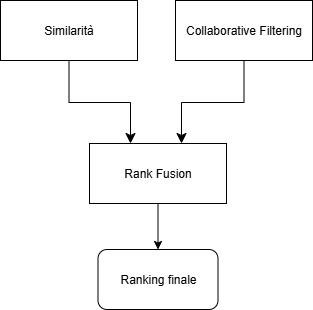
\includegraphics[width=\textwidth]{Diagramma Pipeline sistema di raccomandazione.png}
				\end{figure}
			\end{column}
		\end{columns}
	\end{frame}

	\begin{frame}{Sistema di raccomandazione -\\ Collaborative Filtering}
		Un sistema di \textbf{Collaborative Filtering} sfrutta i comportamenti passati degli utenti per generare raccomandazioni.

		\begin{columns}
			\begin{column}{0.6\textwidth}
				\begin{block}{Principio base}
					\begin{itemize}
						\item Analizza \textbf{preferenze utenti simili}
						\item Identifica \textbf{pattern di acquisto}
						\item Predice \textbf{nuovi interessi}
					\end{itemize}
				\end{block}
			\end{column}
			\begin{column}{0.38\textwidth}
				\begin{figure}
					\centering
					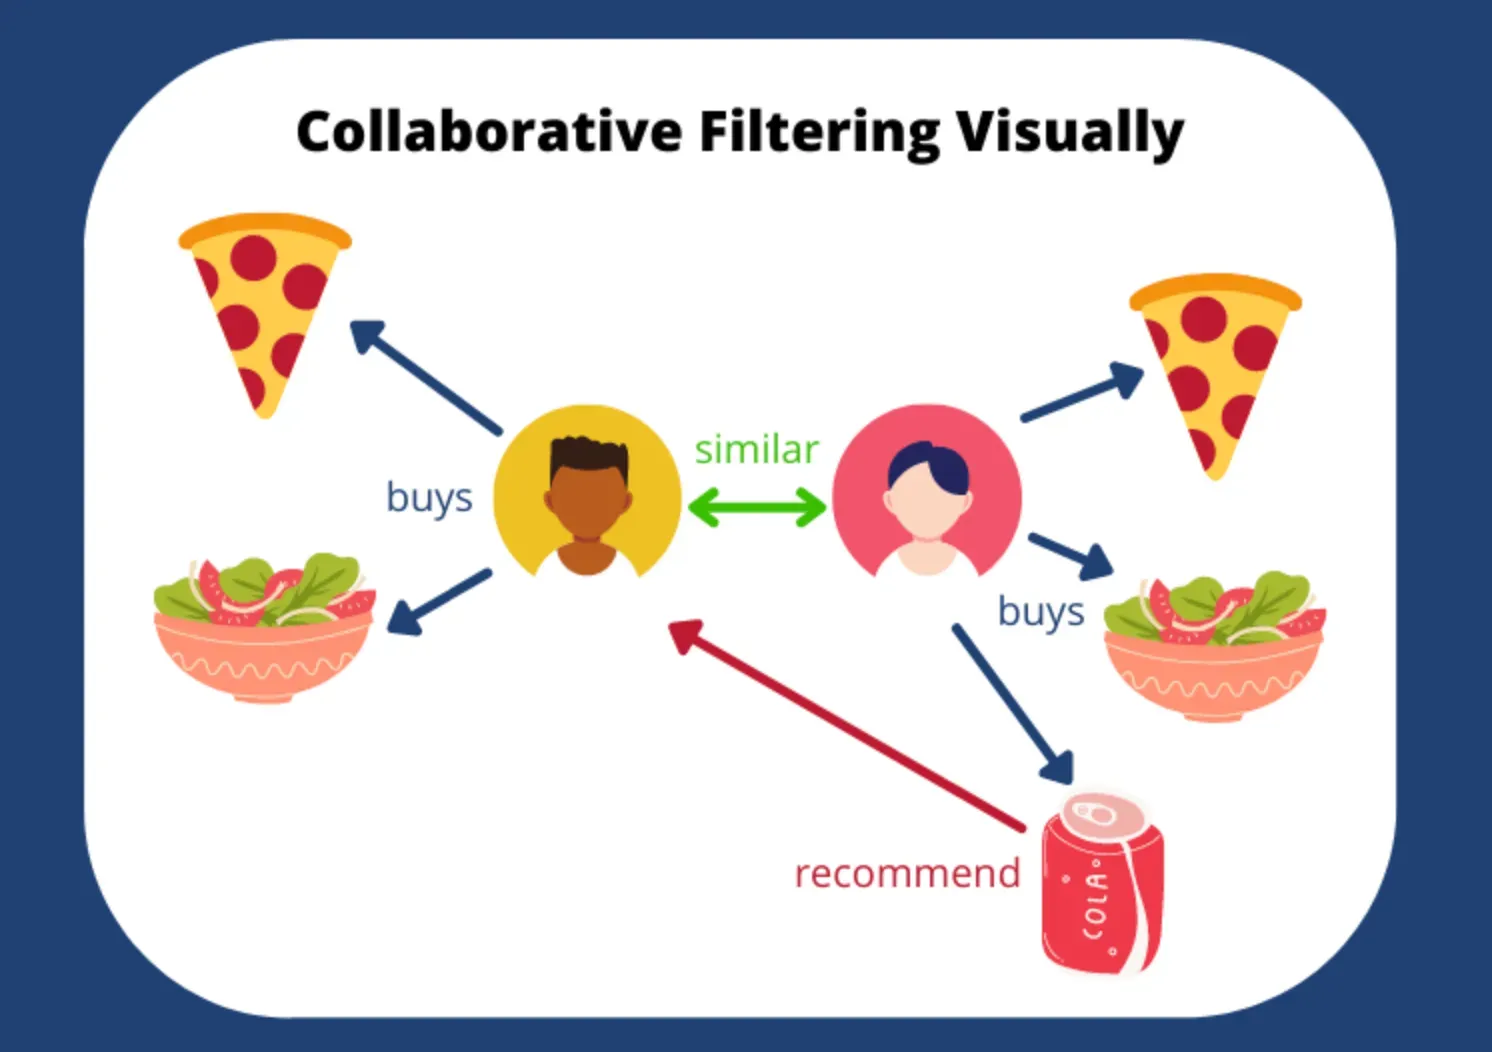
\includegraphics[width=\textwidth]{Collaborative-Filtering.png}
				\end{figure}
			\end{column}
		\end{columns}

		\begin{alertblock}{Logica}
			"Gli utenti con \textbf{gusti simili} nel passato avranno \textbf{preferenze simili} in futuro"
		\end{alertblock}
	\end{frame}

	\begin{frame}{Sistema di raccomandazione - Similarità}
		Un sistema di \textbf{Similarità} sfrutta le caratteristiche semantiche dei prodotti per generare raccomandazioni.

		\begin{columns}
			\begin{column}{0.6\textwidth}
				\begin{block}{Principio base}
					\begin{itemize}
						\item Analizza i \textbf{nomi descrittivi} dei prodotti
						\item Calcola la \textbf{Cosine Similarity}
						\item Identifica i \textbf{prodotti simili}
					\end{itemize}
				\end{block}
			\end{column}
			\begin{column}{0.5\textwidth}
				\begin{figure}
					\centering
					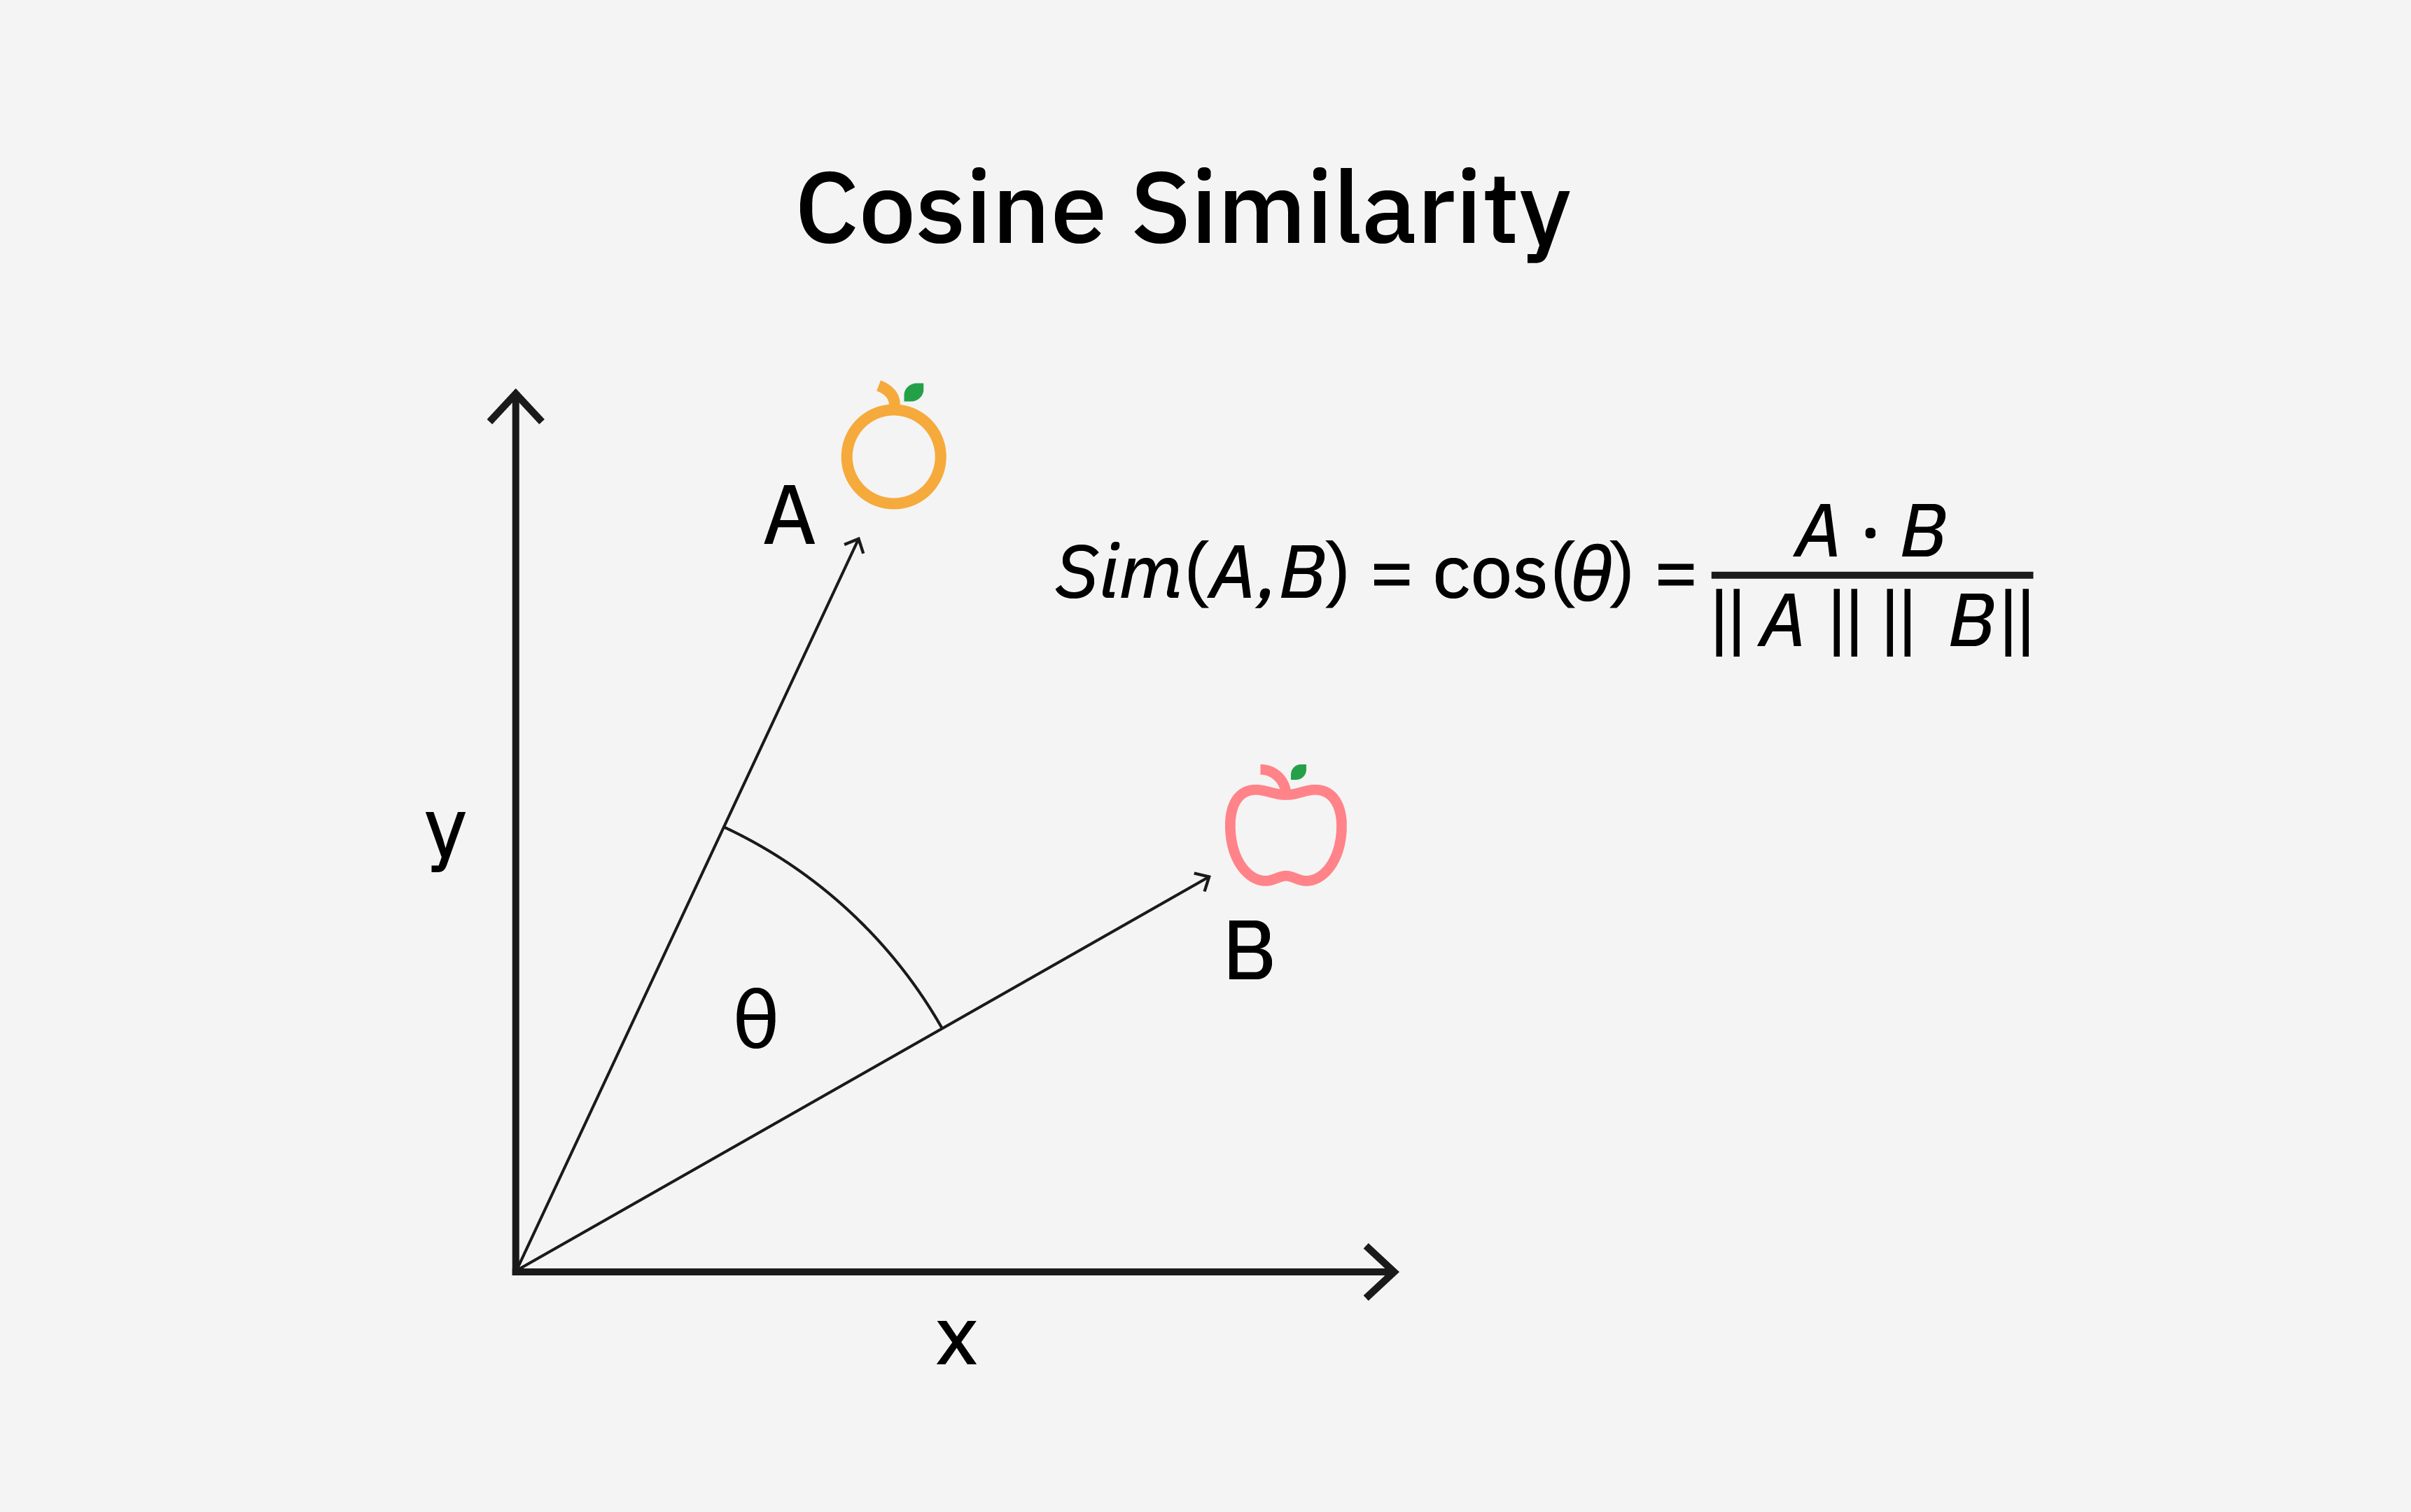
\includegraphics[width=\textwidth]{Cosine-Similarity.png}
				\end{figure}
			\end{column}
		\end{columns}

		\begin{alertblock}{Logica}
			"Se due prodotti hanno \textbf{caratteristiche simili}, le raccomandazioni per uno possono essere \textbf{utili anche per l'altro}"
		\end{alertblock}
	\end{frame}

	\begin{frame}{Sistema di raccomandazione - Formato di archiviazione delle matrici}
        \textbf{Confronto} di \textbf{5 formati} per ottimizzare l'archiviazione matrici:

		\begin{columns}
			\begin{column}{0.6\textwidth}
				\begin{block}{Formati analizzati}
					\begin{itemize}
						\item \textbf{CSV}: Semplice ma inefficiente
						\item \textbf{HDF5}: Form. binario strutturato
						\item \textbf{NPY}: Nativo NumPy veloce
						\item \textbf{Parquet}: Colonnare compresso
						\item \textbf{Zarr}: Array n-dimensionali \textbf{cloud}
					\end{itemize}
				\end{block}
			\end{column}
			\begin{column}{0.4\textwidth}
				\begin{figure}
					\centering
					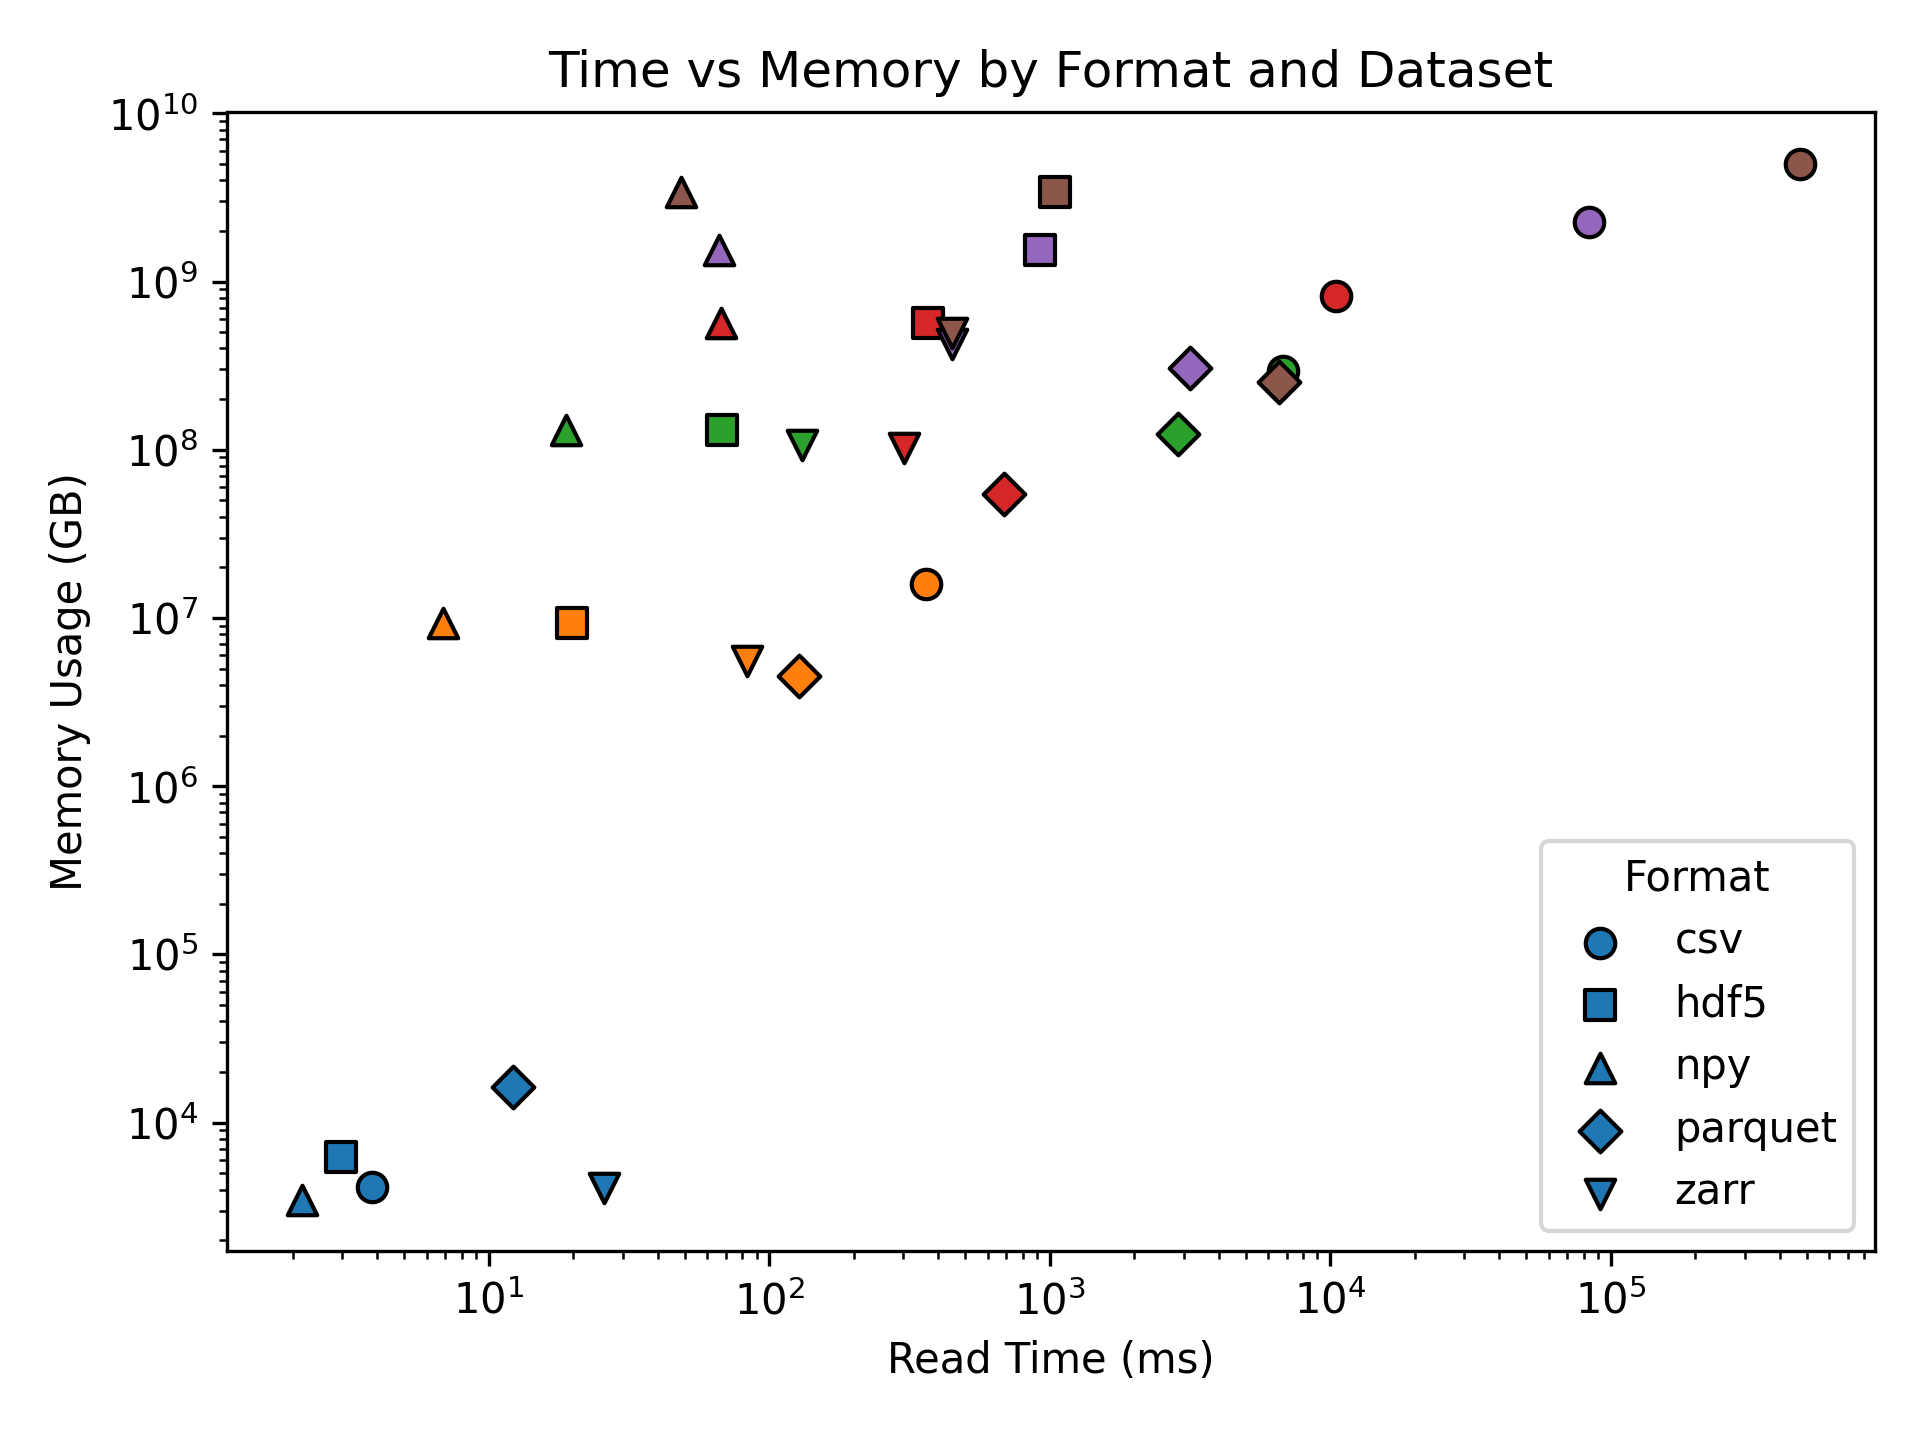
\includegraphics[width=\textwidth]{time_vs_memory.png}
				\end{figure}
			\end{column}
		\end{columns}

		\begin{alertblock}{Risultato}
			\textbf{Zarr} offre il miglior \textbf{compromesso} tra velocità e memoria
		\end{alertblock}
	\end{frame}

	\begin{frame}{Sistema di raccomandazione - Rank Fusion}
		Il \textbf{Reciprocal Rank Fusion (RRF)} combina efficacemente i ranking di diversi sistemi di raccomandazione:

		\begin{columns}
			\begin{column}{0.6\textwidth}
				\begin{block}{Processo RRF}
					\begin{itemize}
						\item \textbf{Input}: Ranking da CF e Similarità
						\item \textbf{Calcolo}: Score reciproco per posizione
						\item \textbf{Fusione}: Somma dei punteggi
						\item \textbf{Output}: Ranking finale unificato
					\end{itemize}
				\end{block}
			\end{column}
			\begin{column}{0.4\textwidth}
				\begin{figure}
					\centering
					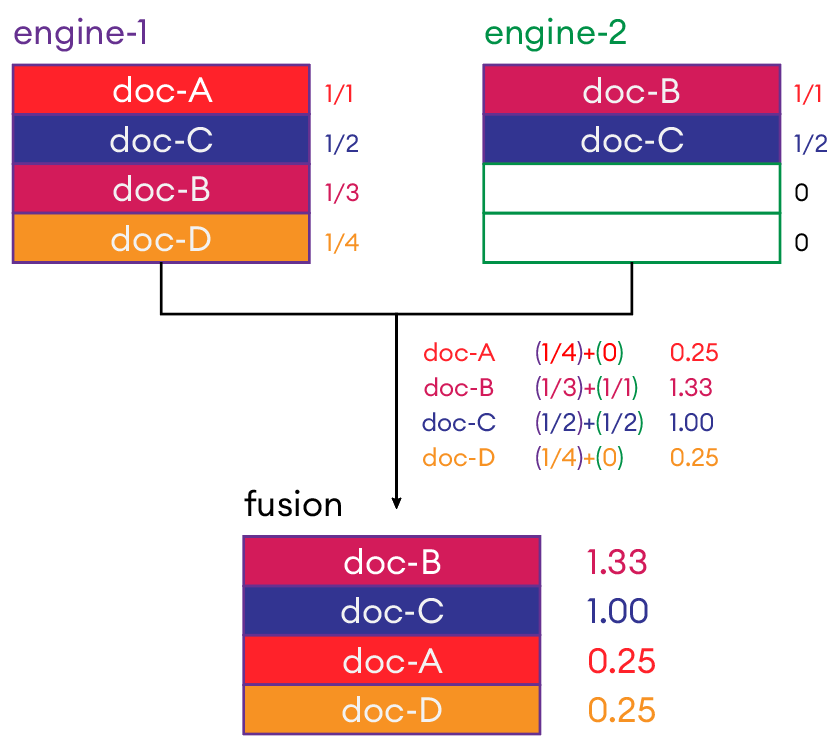
\includegraphics[width=\textwidth]{Reciprocal-Rank-Fusion.png}
				\end{figure}
			\end{column}
		\end{columns}

		\begin{alertblock}{Svantaggio}
			Non considera i punteggi nei ranking di input, solo la loro posizione
		\end{alertblock}
	\end{frame}

	\begin{frame}{Sistema di raccomandazione - Metriche di valutazione}
		Il sistema di raccomandazione è stato valutato utilizzando \textbf{metriche pre-filtro} e \textbf{post-filtro}:

		\begin{columns}
			\begin{column}{0.5\textwidth}
				\begin{exampleblock}{Metriche pre-filtro}
					Valutano le raccomandazioni \textbf{prima} del filtro sui prodotti già acquistati:
					\begin{itemize}
						\item \textbf{Recall@k}
						\item \textbf{Precision@k}
						\item \textbf{MAP@k}
						\item \textbf{MRR@k}
						\item \textbf{Unserendipity@k}
					\end{itemize}
				\end{exampleblock}
			\end{column}
			\begin{column}{0.5\textwidth}
				\begin{exampleblock}{Metriche post-filtro}
					Valutano le raccomandazioni \textbf{dopo} il filtro sui prodotti già acquistati:
					\begin{itemize}
						\item \textbf{Average Item Similarity}
						\item \textbf{Mean Popularity@k}
					\end{itemize}
				\end{exampleblock}
			\end{column}
		\end{columns}
	\end{frame}

	\begin{frame}{Sistema di raccomandazione - Explainability}
		\textbf{Explainability} del sistema di raccomandazione per \textbf{trasparenza decisionale}, disponibile solo per l'\textbf{admin}:

		\begin{alertblock}{Sistema di Explainability implementato}
			\textbf{Logging} di ranking e punteggio in tutte le classifiche generate, per ciascun prodotto o utente raccomandato:
			\begin{itemize}
				\item \textbf{RRF}: ranking e score finale
				\item \textbf{Collaborative Filtering}: ranking e punteggio
				\item \textbf{Similarità}: ranking e punteggio
			\end{itemize}
		\end{alertblock}

		\begin{figure}
			\centering
			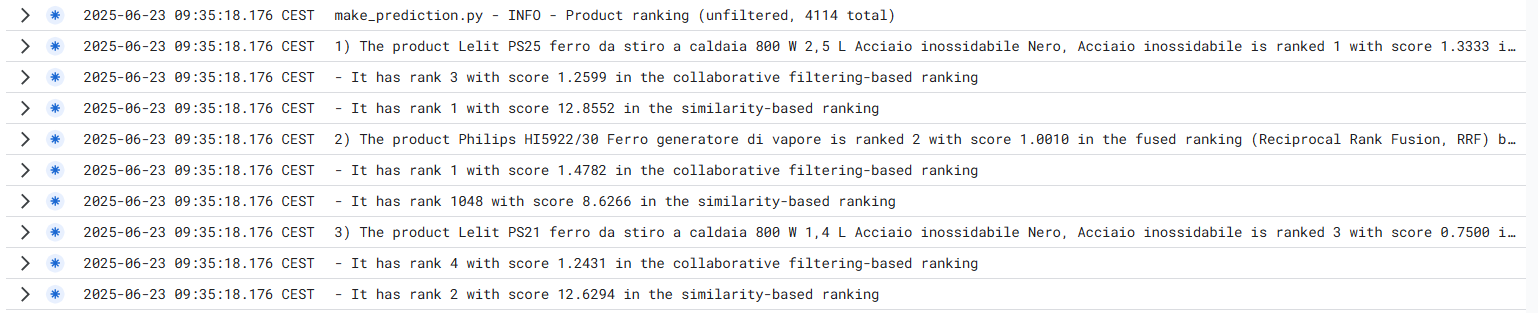
\includegraphics[width=\textwidth]{Explainability - Log della task Recommendation System.png}
		\end{figure}
	\end{frame}


	\section{Deploy e frontend}

	\begin{frame}{Deploy e frontend - Integrazione con\\ Google Cloud}
		\textbf{Integrazione} con \textbf{Google Cloud Platform} per il deployment scalabile e gestione dei dati:

		\begin{columns}
			\begin{column}{0.42\textwidth}
				\begin{exampleblock}{Google Cloud Functions}
					Implementazione di due funzioni serverless: \textbf{sales-analysis} e \textbf{recommendation-system}
				\end{exampleblock}
				
				\begin{figure}
					\centering
					
\includegraphics[width=0.8\textwidth]{Google-Cloud-Functions.png}
				\end{figure}
			\end{column}
			\begin{column}{0.58\textwidth}
				\begin{exampleblock}{Google Cloud Storage}
					Archiviazione delle matrici di raccomandazione generate da \textbf{sales-analysis}, perchè siano prelevabili da \textbf{recommendation-system}
				\end{exampleblock}
				
				\begin{figure}
					\centering
					
\includegraphics[width=0.45\textwidth]{Google-Cloud-Storage.png}
				\end{figure}
			\end{column}
		\end{columns}
	\end{frame}

	\begin{frame}{Deploy e frontend - Interfacce frontend}
		Sviluppo di \textbf{interfacce frontend} dedicate per entrambe le task, cioè sviluppo di \textbf{form} per l'invio dei dati:

		\begin{columns}
			\begin{column}{0.64\textwidth}
				\begin{exampleblock}{Funzionalità}
					\begin{itemize}
						\item \textbf{Integrazione diretta} nel sito dell'e-commerce
						\item \textbf{Validazione} dell'input
						\item Interfaccia \textbf{dedicata}, non generale
						\item Gestione \textbf{dinamica} del submit
					\end{itemize}
				\end{exampleblock}
			\end{column}
			\begin{column}{0.36\textwidth}
				\begin{alertblock}{Tecnologie}
					\begin{itemize}
						\item React
						\item React Hook Form
						\item Zod
						\item Shadcn/ui
					\end{itemize}
				\end{alertblock}
			\end{column}
		\end{columns}

		\begin{figure}
			\centering
			\begin{minipage}{\textwidth}
				\centering
				
\includegraphics[height=1.5cm]{react-logo.jpg}\hspace{0.5cm}
				
\includegraphics[height=1.5cm]{react-hook-form-logo.jpg}\hspace{0.5cm}
				
\includegraphics[height=1.5cm]{zod-logo.jpg}\hspace{0.5cm}
				
\includegraphics[height=1.5cm]{shadcn-ui-logo.png}
			\end{minipage}
		\end{figure}
	\end{frame}


	\section{Ottimizzazione}

	\begin{frame}{Ottimizzazione}
		\textbf{Ottimizzazione} del preprocessing per \textbf{migliorare le performance}:

		\begin{columns}
			\begin{column}{0.5\textwidth}
				\begin{block}{Miglioramenti}
					\begin{itemize}
						\item Introduzione delle \textbf{Pandas Vectorized Ops}
						\item Eliminazione delle operazioni \textbf{pandas.DataFrame.apply}
						\item Miglioramento dell'algoritmo delle \textbf{etichette}
					\end{itemize}
				\end{block}
			\end{column}
			\begin{column}{0.5\textwidth}
				\begin{exampleblock}{Risultati nei dataset testati}
					\begin{itemize}
						\item \textbf{Generale miglioramento} dei tempi di esecuzione
						\item Miglioramento \textbf{medio} del \textbf{20\%}
						\item Miglioramento \textbf{massimo} vicino al \textbf{40\%}
					\end{itemize}
				\end{exampleblock}
			\end{column}
		\end{columns}

		\begin{figure}
			\centering
			\includegraphics[width=0.65\textwidth]{Tabella risultati ottimizzazione - I miglioramenti più significativi.png}
		\end{figure}
	\end{frame}


	\section{Conclusioni e considerazioni finali}

	\begin{frame}{Conclusioni e considerazioni finali}
		Il periodo di \textbf{stage} presso Oribea si è concluso con \textbf{successo}, raggiungendo \textbf{tutti gli obiettivi} prefissati e \textbf{migliorando la Business Intelligence} delle aziende clienti delle task.

		\begin{columns}
			\begin{column}{0.48\textwidth}
				\begin{block}{Risultati ottenuti}
					\begin{itemize}
						\item Implementata task di \textbf{analisi vendite}
						\item Implementata task di \textbf{raccomandazione}
						\item Sviluppate \textbf{interfacce frontend} per collegamento diretto da sito e-commerce
					\end{itemize}
				\end{block}
			\end{column}
			\begin{column}{0.52\textwidth}
				\begin{alertblock}{Sviluppi futuri}
					\begin{itemize}
						\item \textbf{Chatbot} per unire le due task
						\item Sistema di \textbf{logging avanzato}
						\item Introduzione della \textbf{serendipità} nelle raccomandazioni
						\item \textbf{Data reduction} per ridurre le dimensioni delle matrici
					\end{itemize}
				\end{alertblock}
			\end{column}
		\end{columns}
	\end{frame}

	\begin{frame}{Domande?}
		\begin{center}
			\Large
			\textbf{Grazie per l'attenzione!}
			
			\vspace{1em}
			
			\normalsize
			\textit{Presentazione disponibile su:}\\
			\url{https://github.com/Rickyz03/Presentazione-Discussione-LT-Informatica}
			
			\vspace{2em}
			
			\Large
			\textbf{Ci sono domande?}
		\end{center}
	\end{frame}


\end{document}
